\documentclass[a4paper,12pt]{scrbook}
\usepackage[bookmarks=true,colorlinks=true]{hyperref} 
\hypersetup{
 pdfauthor = {Alexander Wiebel},
 pdftitle = {OpenWalnut Design},
 pdfsubject = {Design Document},
 pdfkeywords = {Visualization System, Medical Visualization},
 pdfcreator = {LaTeX with hyperref package},
 pdfproducer = {pdflatex}}

\usepackage[latin1]{inputenc}
\usepackage{color}
\usepackage{graphicx}
\usepackage{pst-grad,pstricks}
\usepackage{amsmath}
\usepackage{amssymb}
\usepackage{amsfonts}
\usepackage{subfigure}
\usepackage{wrapfig}
\bibliographystyle{alpha} 

\newcommand{\todo}[1]{\textcolor{white}{\colorbox{red}{\\ Noch zu %
      tun:}}\ \ #1 \textcolor{red}{\colorbox{red}{I}}\\\ \\\ }
\newcommand{\here}{\textcolor{white}{\colorbox{red}{\\\LARGE HIER}} }

\begin{document}
\titlehead{
  OpenWalnut Project\\
  www.openwalnut.org}

\subject{Documentation}
\title{
  OpenWalnut Design
}
\author{ Alexander Wiebel }
\publishers{Leipzig}
\maketitle

\tableofcontents

\chapter{Introduction}
\section{Class Diagrams}
We use UML type notation in diagrams describing relationships between classes. Some of the descriptions used throughout this
section stem from the following website:
\begin{itemize}
\item \verb|http://en.wikipedia.org/w/index.php?title=Class_diagram&oldid=314998859|
\end{itemize}


\begin{figure}[htb]
  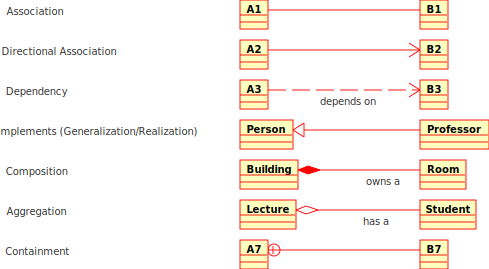
\includegraphics[width=\textwidth]{relationship_examples}
  \caption{Examples for relationships used in class diagrams.}
\end{figure}


\begin{description}
\item[Aggregation] can occur when a class is a collection or container of other classes, but where the contained classes do not
  have a strong life cycle dependency on the container -- essentially, if the container is destroyed, its contents are not.
\item[Composition] usually has a strong life cycle dependency between instances of the container class and instances of the
  contained class(es): If the container is destroyed, normally every instance that it contains is destroyed as well.
\end{description}
\chapter{Math}


\begin{figure}[htb]
  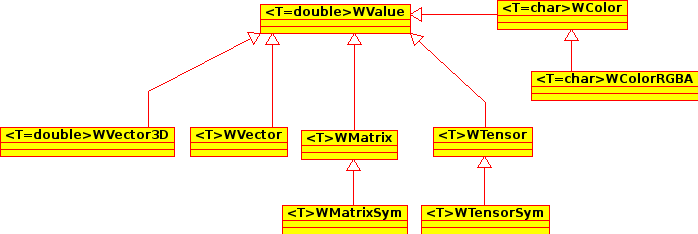
\includegraphics[width=\textwidth]{WValue_hierachy}
  \caption{The class hierarchy describing high-level values in OpenWalnut.}
\end{figure}
\section{Literature}
For a general overview on visualization in medicine \cite{Preim:2007:VMT} can be recommended.

\chapter{GUI}
The GUI module is the only part where we allow gui-toolkit related code. For example, this means that the use of any QT class is
prohibited outside the GUI module.
\chapter{GE (Graphics Engine)}
The graphics engine is mainly realized by integrating OpenSceneGraph (OSG) so far.
\chapter{DataHandler}
This chapter describes the main ideas of the architecture of our module that implements the data handling. WDataHandler is the
main entry point to the module. It contains all subject's data present in OpenWalnut. The data set belonging to a subject are held by
an instance of WSubject. Each of the data sets of a subject is encapsulated by a WDataSet object. 

\begin{figure}[htb]
  \centering
  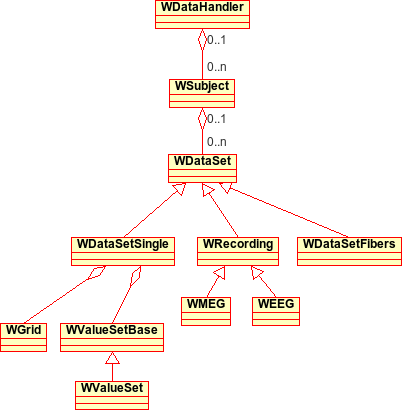
\includegraphics[width=.4\textwidth]{dataHandler_classDiagram}
  \caption{Class diagram describing the data handler's architecture.}
\end{figure}

WDataSet is the base class for a number of subclasses representing different types of data sets, e.g.
\begin{itemize}
\item WDataSetSingle - A simple single data set.
\item WDatSetTimeDependent - A data set that encapsulates a number of data sets for different time steps.
\end{itemize}

\section{Data Sets}
The subsections in this section are organized according to different types of recording or imaging data.
\subsection{EEG}
\subsubsection{Note}
sread in BIOSIG C++ toolbox provides start and length parameters ... these should be used as EEG might not fit or at least is not
intended to be completely in the main memory. This should also be reflected in the design of the data structure.  Is segment-wise
loading a good solution?

\subsection{Image Data}

A WDataSetSingle is a WDataSet and has a WValueSet and a WGrid.

A WDataSetTimeDependent is a WDataSet has more than one WValueSet and at least one WGrid (at the moment, i.e. 2009-05-13 we expect
only one WGrid)

A WValueSet has subclasses for different types of values.

\section{Raw Access}
Certain types of data sets provide a low level access for the GraphicsEngine to ensure performance. This access is realized by a
function similar to
\begin{verbatim}
T* getValuesPointer< class T >()
\end{verbatim}
and code to get the access then looks similar to
\begin{verbatim}
float *myValuePointer;
myValuePointer = getValuesPointer<float *>()
\end{verbatim}

\section{Enforced rules}
\begin{itemize}
\item Data can not be manipulated!
\end{itemize}

\bibliography{../../books}
\end{document}
